\section{Описание работы}
Подготовить исходные данные с помощью программы Avogadro. Провести оптимизация геометрии (Energy Optimization) с помощью программы GAMESS. Проанализировать результаты.

Расчитываемая молекула: этиленгликоль $C_2H_4 - (OH)_2$

\begin{figure}[H]
\centering
\captionsetup{justification=centering}
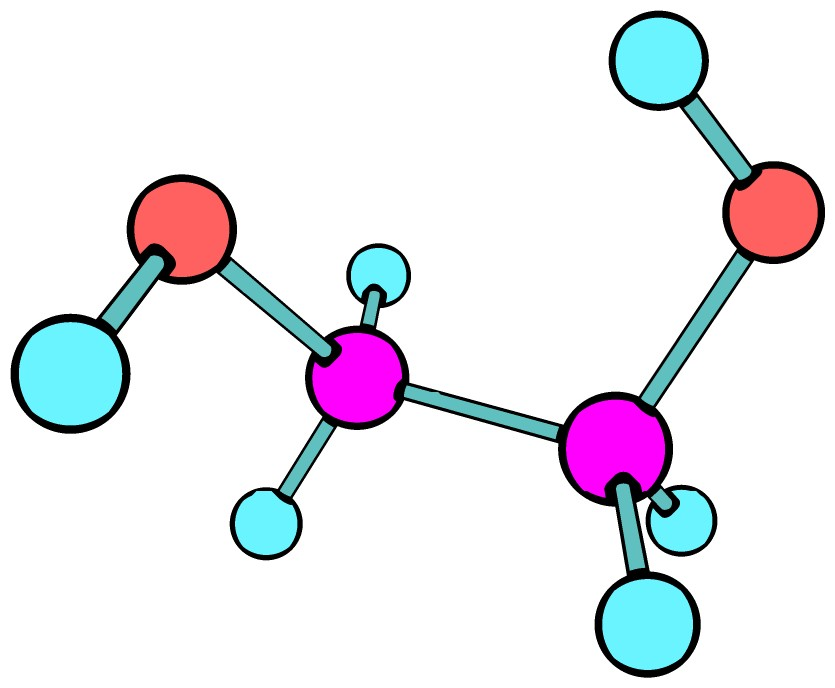
\includegraphics[scale=0.4]{fig/0.jpg}
\caption{Изопропанол. Цветами обозначены атомы: голубой - водород, фиолетовый - углерод, красный - кислород.}
\end{figure}

\newpage
\section{Постановка задачи}
Предварительно оптимизировать молекулярную структуру с помощью программы Avogadro, затем провести геометрическую оптимизацию с помощью программы GAMESS методом DFT. Проанализировать следующие показатели: 
\begin{itemize}
    \item номер слейтеровской орбитали, локализованной на атоме кислорода, которая вносит существенный вклад в HOMO;
    \item определить заселенность по Малликену атомов кислорода и максимальную межатомную заселенность;
    \item привести исходное значение полной энергии (в а.е.) до начала процесса оптимизации и полную энергию, полученную после завершения процесса оптимизации геометрии. Для полной энергии, полученной по окончанию оптимизации, привести вклады электронной энергии и энергии кулоновского отталкивания ядер.
    \item сопоставить геометрии (длины связей) до и после оптимизации, визуализировать результат.
\end{itemize}

\newpage
\section{Теоретическая информация}
\subsection{Теория функционала плотности}
ТФП связывает свойства молекулярных систем с электронной плотностью основного состояния\footnote{Для исследования возбужденных состояний можно использовать TD DFT или TD HF} и опирается на теорему Хоэнберга—Кона, которая утверждает, что энергия системы есть функционал электронной плотности, а точная электронная плотность основного состояния обеспечивает минимум энергии:

\begin{equation}
    E[\rho] = -\frac{1}{2}\sum\limits_i\nabla^2\psi_i(\Vec{r}) + \int V_{я}(\Vec{r})\rho(\Vec{r}) + \frac{1}{2}\int\int\frac{\rho(\Vec{r})\rho(\Vec(r')}{|\Vec{r} - \Vec{r'}|}d\Vec{r}d\Vec{r'} + E_{xc}[\rho]
\end{equation}

Различные методы ТФП отличаются друг от друга выбором обменно-корреляционного функционала. Один из наиболее популярных методов является гибридный метод B3LYP, в котором смешаны различные другие методы ТФП. 

\newpage
\section{Результаты}
\subsubsection*{Определить номер HOMO, которая содержит существенный вклад АО, локализованной на атоме кислорода.}
Номер HOMO 17. Наиболее существенный вклад вносит $2p_z$-орбиталь (-0.537052), центрированная на атоме O2 (раздел EIGENVECTORS).
\subsubsection*{Анализ заселенностей атомов O1 и O2}
\begin{figure}[H]
\centering
\captionsetup{justification=centering}
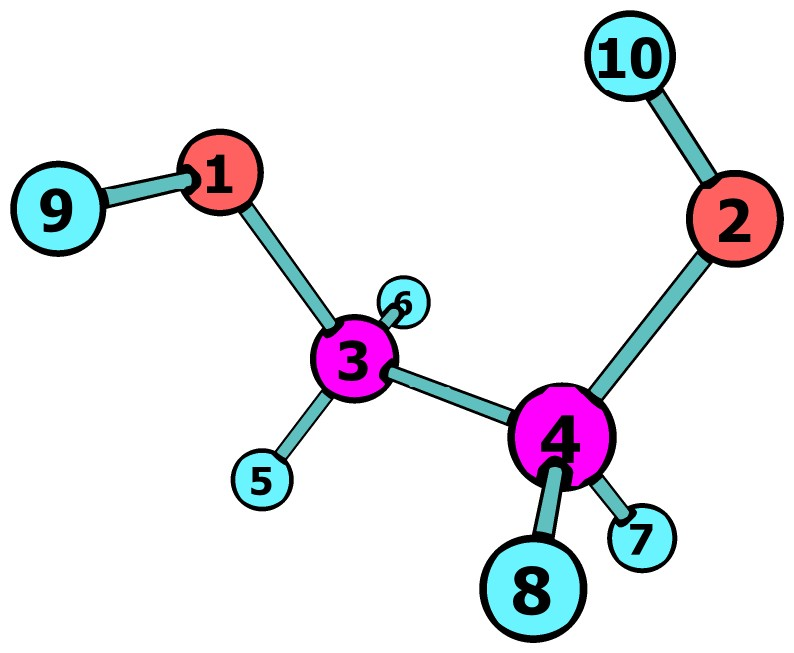
\includegraphics[scale=0.4]{fig/1.jpg}
\caption{Номера атомов в молекуле этиленгликоль. Цветами обозначены атомы: голубой - водород, фиолетовый - углерод, красный - кислород.}
\end{figure}

Полная заселенность по Малликену для атомов O1 и O2 составялет 8.6.Так как заряд ядра атома кислорода составялет +8, то в данном соединении кислород является электроотрицательным. Максимальная межатомная заселенность образована между атомами С3-H6 -- 0.745322 (разделы TOTAL MULLIKEN AND LOWDIN ATOMIC POPULATIONS и MULLIKEN ATOMIC OVERLAP POPULATIONS). 
\subsubsection*{Сопоставление полной энергии}
Была проведена оптимизация геометрии методом B3LYP в базисе 6-31G.

\begin{table}[H]
\caption{Значения составляющих полной энергии для молекулы до и после проведения оптимизации (в Хартри)} \label{tab:my-table}
    \begin{center}
        \begin{tabular}{|c|c|c|}
        \hline
         & До оптимизация & После оптимизации \\ \hline
        \begin{tabular}[c]{@{}c@{}}Кинетическая энергия\\ электронов\end{tabular} & 229.082 & 228.911 \\ \hline
        \begin{tabular}[c]{@{}c@{}}Электрон-электронное\\ взаимодействие\end{tabular} & 214.520 & 213.127 \\ \hline
        \begin{tabular}[c]{@{}c@{}}Электрон-ядерное\\ взаимодействие\end{tabular} & -807.080 & -803.973 \\ \hline
        \begin{tabular}[c]{@{}c@{}}Ядер-ядерное\\ взаимодействие\end{tabular} & 133.435 & 131.889 \\ \hline
        \textbf{Полная энергия} & \textbf{-230.042} & \textbf{-230.045} \\ \hline
        \end{tabular}
    \end{center}
\end{table}

Изменение полной энергии составило менее 1\%, что является несущественным. Это значит, что Avogadro хорошо проводит оптимизацию.
\subsubsection*{Сопоставление длин связей}
Была проведена оптимизация геометрии методом B3LYP в базисе 6-31G.

\begin{figure}[H]
\centering
\captionsetup{justification=centering}
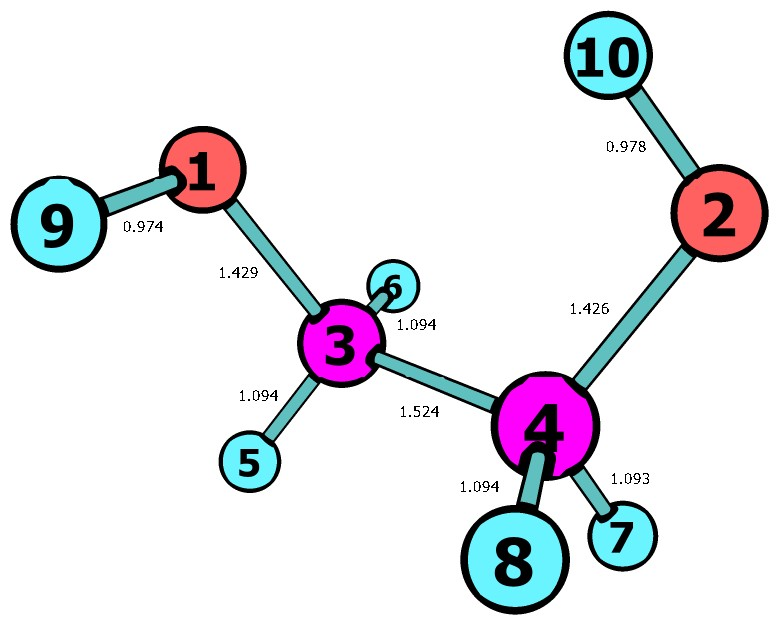
\includegraphics[scale=0.4]{fig/2.jpg}
\caption{Геометрия молекулы до оптимизации}
\end{figure}

\begin{figure}[H]
\centering
\captionsetup{justification=centering}
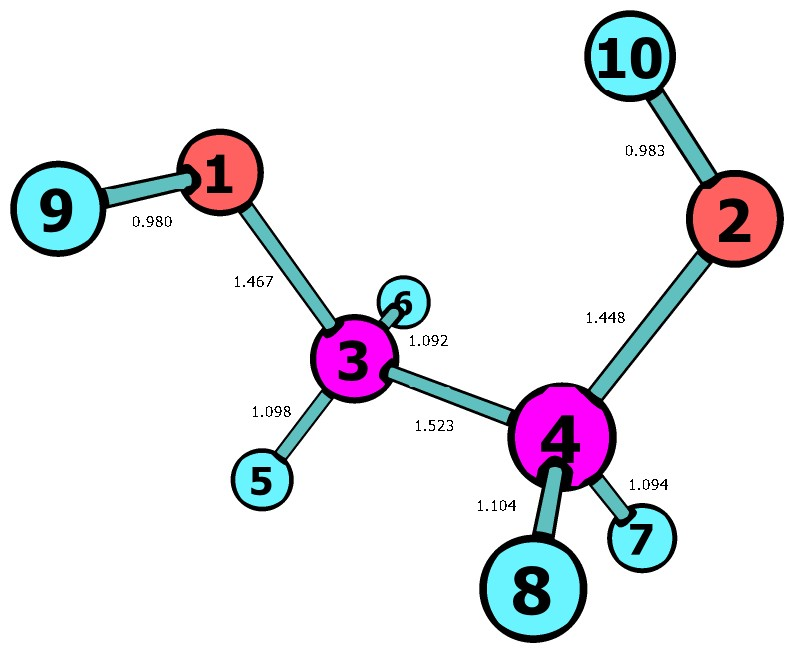
\includegraphics[scale=0.4]{fig/3.jpg}
\caption{Геометрия молекулы после оптимизации}
\end{figure}

\begin{table}[H]
\caption{Длины связей в молекуле до и после оптимизации}
\label{tab:tab4}
\begin{center}
\begin{tabular}{|c|c|c|c|}
\hline
\multirow{2}{*}{Связь} & \multicolumn{2}{c|}{Длина связи} & \multirow{2}{*}{\begin{tabular}[c]{@{}c@{}}Относительная \\ разница, \%\end{tabular}} \\ \cline{2-3}
 & До оптимизации & После оптимизации &  \\ \hline
O1-H9 & 0.974 & 0.980 & 0.62 \\ \hline
O1-C3 & 1.429 & 1.467 & 2.66 \\ \hline
C3-H5 & 1.094 & 1.098 & 0.37 \\ \hline
C3-H6 & 1.094 & 1.092 & -0.18 \\ \hline
C3-C4 & 1.524 & 1.523 & -0.07 \\ \hline
C4-H8 & 1.094 & 1.104 & 0.91 \\ \hline
C4-H7 & 1.093 & 1.094 & 0.09 \\ \hline
C4-O2 & 1.426 & 1.448 & 1.54 \\ \hline
O2-H10 & 0.978 & 0.983 & 0.51 \\ \hline
\end{tabular}
\end{center}{}
\end{table}

Как видно из таблицы, наиболее существенно изменилась связь O1-C3.

\newpage
\section{Контроль результатов}
Процесс оптимизации геометрии в расчете действительно завершен (в выходном файле содержится: ''EQUILIBRIUM GEOMETRY LOCATED''). В результате расчета получена геометрия с более низкой полной энергией, чем после предварительной оптимизации в Avogadro.

Приложенные файлы:
\begin{itemize}
    \item Ethylene\_glycol.inp – исходные данные GAMESS для расчета методом DFT (B3LYP) в базисе 6-31G;
    \item Ethylene\_glycol.log – результат расчета методом DFT (B3LYP) в базисе 6-31G;
\end{itemize}{}